%\documentclass[]{diss}
%\begin{document}
\chapter{A whole systems approach to processing}
\label{s:german-locative-phrases-syntax-semantics-integration}
So far I have discussed processing of German locative phrases
isolated for semantics and syntax. However, IRL and FCG are systems that 
have to work together to allow agents to talk. This chapter reflects on the 
integration of these two systems in a unified architecture. 
Consequently this chapter is technical in nature. It starts out by giving
an overview of how processing is integrated (Section \ref{s:irl-fcg-integration}).
Section \ref{s:semantic-ambiguity} discusses the phenomenon of 
semantic ambiguity\index{semantic ambiguity} which requires a deep level of integration.
The chapter concludes with results on the performance of the 
complete system (Section \ref{s:syntax+semantics-integration}).


\section{Integrating IRL and FCG}
\label{s:irl-fcg-integration}
IRL and FCG are integrated via a mechanism which is called 
\textsc{task engine}.\footnote{All computational systems described in this 
book are integrated into a framework for running and evaluating 
experiments described in \cite{steels2010babel}\index{Steels, L.}\index{Loetzsch, M.}.}
The task engine bundles the processing done by an agent and allows to track
different hypotheses. For instance, in production a speaker might conceptualize
different semantic structures and only later decide which of those he wants
to use based on how well it can be verbalized. For this IRL and FCG 
is packaged into processes.\index{task processor}

\begin{figure}
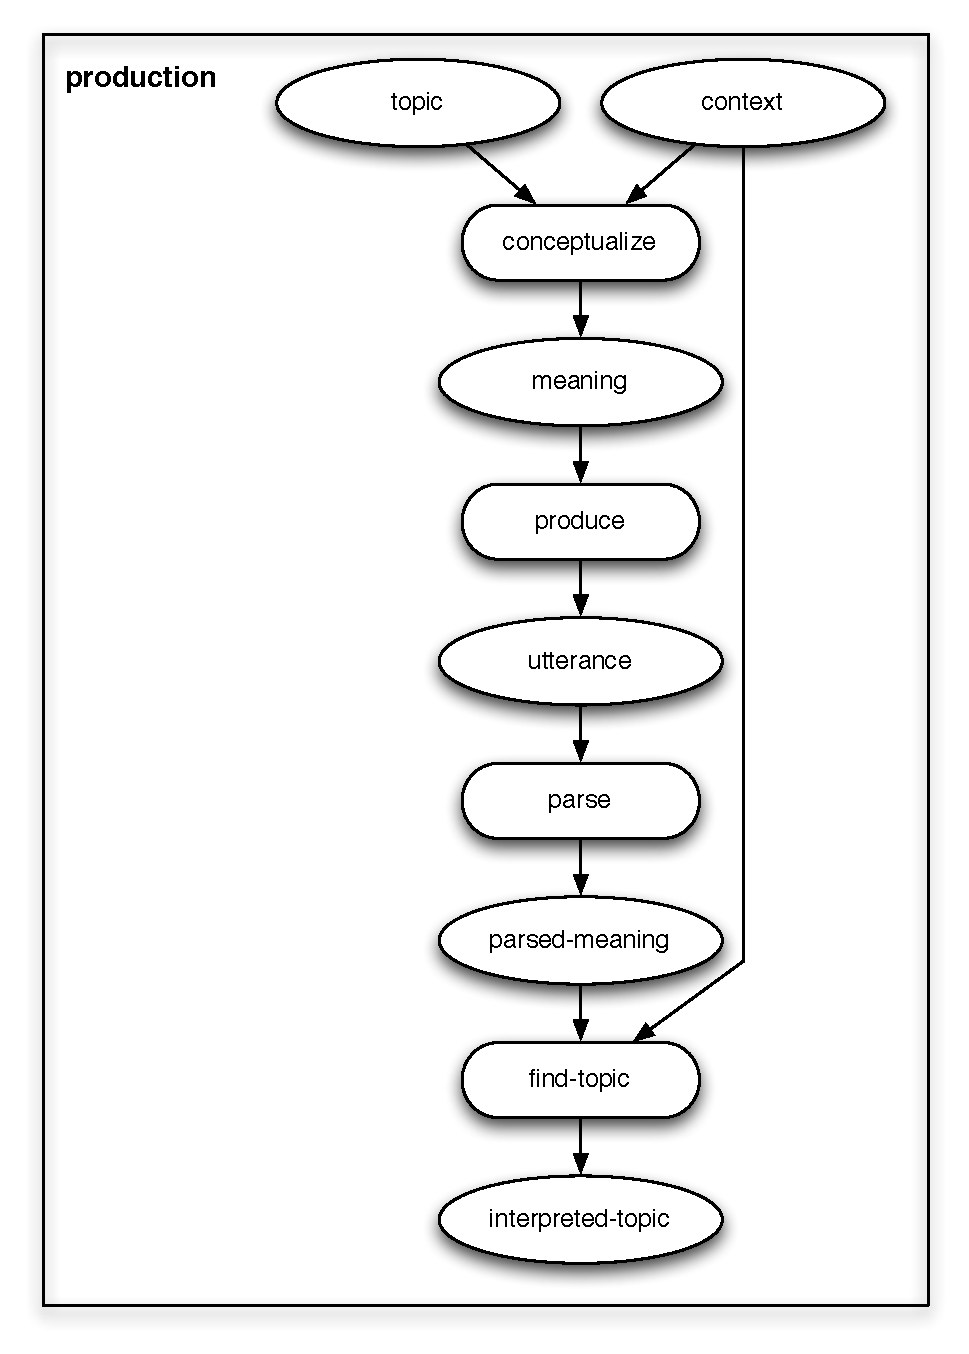
\includegraphics[width=0.5\textwidth]{figs/production}
\caption[Processes running when a speaker produces an utterance]{%
Processes running when a speaker produces an utterance. Ellipsis represent
data structures, squashed rectangles represent processes.}
\label{f:production}
\end{figure}

Figures~\ref{f:production} and~\ref{f:interpretation} show the typical processing 
for the speaker and the hearer.
Each of them runs different processes which bundle FCG 
and IRL for production and interpretation. The most 
important processes are 
\begin{description}
\item[conceptualize] This process takes as input the world model (context) computed 
by the vision system and a topic object. Using these input 
arguments, an ontology and a set of known chunks, the process uses the 
IRL search to produce one or several possible IRL-networks.
\item[produce] This process applies constructions in the direction of production.
In other words, matching happens on the semantic side. Production takes as input
an IRL-network and a set of constructions and produces one or more possible utterances
using FCG's search process.
\item[parse] Parsing is the process which takes a set of constructions as well as an utterance
and computes one or more possible interpretations, i.e. IRL-networks.
\item[find-topic] This process uses IRL to compute a topic based on 
an IRL-network and the context (computed by the vision system).
\end{description}
All of these processes can produce one or many outcomes. The task engine
branches on multiple results. For instance, when ``conceptualize'' has found
different IRL-networks, the engine tracks their individual success in separate 
``produce'' processes. The overall best result is determined by 
combining the discrimination score of the meaning and confidence of construction 
application. Moreover, as we can see in \figref{f:production}, speakers also run processes vital 
for the hearer. Before passing an utterance to the hearer, the speaker parses and
interprets the phrase he is about to use. The mechanism is called 
\textsc{re-entrance}\index{re-entrance} \citep{steels03reentrance}\index{Steels, L.}. Applied to this process model,
this means that agents can choose the best result based on the 
prediction how that phrase might be interpreted by the hearer.

\begin{figure}
\begin{center}
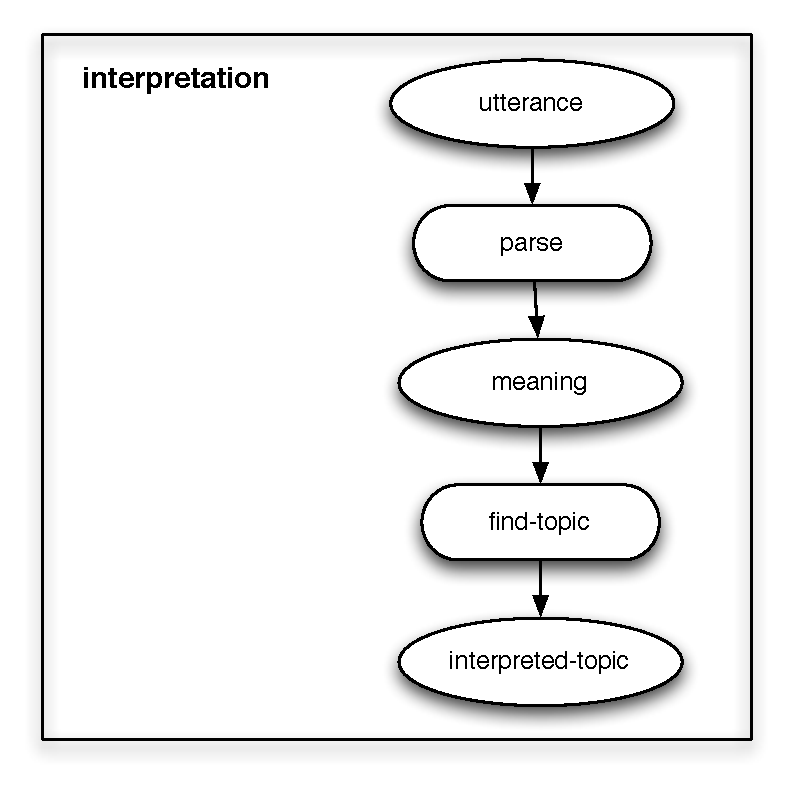
\includegraphics[width=0.5\textwidth]{figs/interpretation}
\caption[Processes running when a hearer interprets an utterance]{%
Processes running when a hearer interprets an utterance. Ellipsis represent
data structures, squashed rectangles represent processes.}
\label{f:interpretation}
\end{center}
\end{figure}

\section{Handling semantic ambiguity}\index{semantic ambiguity}
\label{s:semantic-ambiguity}
An example where the integration of the systems for syntactic processing
and conceptualization can play out its power is semantic ambiguity.
A phrase is semantically ambiguous if multiple semantic structures, i.e. IRL-networks,
can be interpreted. 

% german locative phrases - syntactic and semantic ambiguity
Many German locative phrases are semantically ambiguous.
Let us consider the following two examples from German.
\ea
\label{e:der-block-vor-der-linken-kiste}
\gll der Block vor der linken Kiste\\
the.{\NOM} block.{\NOM} front.{\PREP} the.{\DAT} left.{\ADJ}.{\DAT} box.{\DAT}.{\textsc{fem}}\\ 
\glt `The block in front of the left box'\\
%\glend
\item
\label{e:der-block-vor-der-linken-kiste-von-dir-aus}
\gll der Block vor der linken Kiste von dir aus \\
the.{\NOM} block.{\NOM} front.{\PREP} the.{\DAT} left.{\ADJ}.{\DAT} box.{\DAT} from.{\PREP} your.{\DAT}  perspective\\
\glt `The block in front of the left box from your perspective'\\
%\glend
\z
\REF{e:der-block-vor-der-linken-kiste} is semantically ambiguous with 
respect to how the landmark object, in this case the left box, is 
conceptualized. The phrase can have an intrinsic or relative reading.
\REF{e:der-block-vor-der-linken-kiste-von-dir-aus} does not have this problem. 
The perspective marker clearly signals a relative reading of the phrase.
Interestingly, this fact can only be established after parsing the complete phrase. 
To illustrate this dependency consider \REF{e:der-block-vor-der-linken-kiste-von-dir-aus}, 
which is not semantically ambiguous (with respect to intrinsic and relative readings)
because it features a perspective marker in the end. 

The first example is a clear instance of language as an inferential coding 
system \citep{sperber1986relevance}\index{Wilson, D.}\index{Sperber, D.}. Utterances merely hint at meaning 
rather than encoding complete information.
In other words, the information communicated in utterances is incomplete and
ambiguous. This puts considerable stress on hearers, as it requires them
to integrate information from the context with the information available in the
utterance to find the best possible interpretation of a phrase.
The integration of IRL and FCG supports such active information integration
and enables hearers to infer the communicative intention of speakers
even when the information conveyed in the utterance is sparse, incomplete,
and ambiguous. 

This section first discusses the syntactic processing part 
(Section \ref{s:semantic-ambiguity-syntactic}), before examine how 
syntactic processing and semantic processing 
interact (Section \ref{s:semantic-ambiguity-semantic}).


\subsection{Syntactic processing}
\label{s:semantic-ambiguity-syntactic}
The main task of FCG in cases of semantic ambiguity\index{semantic ambiguity} is to correctly 
retrieve the possible interpretations of a phrase. For instance, if there
is a relative and an intrinsic reading of a phrase then those two 
readings should be recovered in parsing -- not more, but also not less.

This section shows how to handle phrases such as in  
\REF{e:der-block-vor-der-linken-kiste} and \REF{e:der-block-vor-der-linken-kiste-von-dir-aus}
using a combination of these techniques:
\begin{enumerate}
\item {logic variables}, for representing uncertainty
\item {percolation}, for distributing information
\item {the actual-potential design pattern}\index{design pattern!actual-potential}, for constraining the 
application of constructions
\item {sem-sem constructions}, which are particular constructions 
that only apply on the semantic side of 
feature structures, for postponing decisions
\end{enumerate}
When applied together, this set of techniques allows to represent 
the inherent ambiguity in certain German locative phrases in a 
concise way, while allowing constructions to collectively resolve the ambiguity 
where possible, or to otherwise interpret the phrase in all possible ways.

The semantic ambiguity\index{semantic ambiguity} discussed in this chapter 
focuses entirely on how a particular landmark is conceptualized.
Consequently, such kind of ambiguity only surfaces in phrases involving 
overtly or covertly expressed landmarks. Examples
of such phrases are prepositional and adverbial phrases, such as 
the following (\REF{e:der-block-vorne} is repeated 
in \REF{e:der-block-vorne-repeated} 
for convenience):
\ea
\label{e:der-block-vorne-repeated}
\gll der Block vorne\\
the.{\NOM} block.{\NOM} front.{\ADV} \\
\glt `The block in front'\\
%\glend
\item
\label{e:der-block-links-von-der-kiste}
\gll der Block links von der Kiste \\
the.{\NOM} block.{\NOM} left.{\ADV} of.{\PREP} the.{\DAT} box.{\DAT} \\
\glt `The block to the left of the box'\\
%\glend
\item
\label{e:der-block-hinter-der-kiste}
\gll der Block hinter der Kiste  \\
the.{\NOM} block.{\NOM} hinter.{\PREP} the.{\DAT} box.{\DAT} \\
\glt `The block in back of the box'\\
%\glend
\z
\REF{e:der-block-links-von-der-kiste} and \REF{e:der-block-hinter-der-kiste} 
explicitly refer to the landmark object, whereas 
\REF{e:der-block-vorne-repeated} implicitly refers to a landmark. 
In all examples, a projective term is used in relation with some landmark, 
denoting the particular spatial relationship of the object
in question, in this case the block, to the landmark. 
Also in all examples, the landmark can be construed using an intrinsic or 
relative frame of reference. Hence, all of the examples have at least two 
possible interpretations.

Syntactic structure can provide additional information that allows
for the disambiguation of the conceptualization underlying a particular utterance. 
This is the case when the phrase also features a perspective marker, 
such as in \REF{e:der-block-vor-der-kiste-von-dir-aus}.
\ea
\label{e:der-block-vor-der-kiste-von-dir-aus}
\gll der Block vor der Kiste von dir aus \\
the.{\NOM} block.{\NOM} front.{\PREP} the.{\DAT} box.{\DAT} from.{\PREP} your.{\DAT} from.{\PREP}\\
\glt `The block in front of the box from your perspective'\\
%\glend
\z\todo{Please re-consider glossing in this and similar examples}
The component \textit{von dir aus} (`from your perspective') is a clear indicator that
the landmark is construed from a certain perspective. Consequently, this phrase 
has a relative reading only. After all, interpreting a relative landmark always entails 
construing the scene from a certain perspective.
This excludes intrinsic readings of the phrase, since construing 
a landmark using an intrinsic frame of reference is independent of the viewpoint of the scene. 

The interaction with perspective marking makes the semantic 
ambiguity in German locative phrases an interesting problem
because whether a phrase is semantically ambiguous can only be established upon
integrating information from the complete phrase.

\begin{figure}
\begin{center}
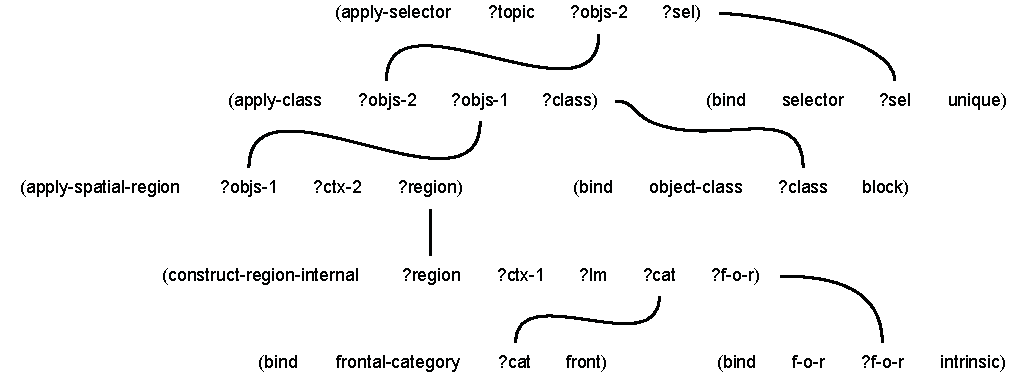
\includegraphics[width=.8\textwidth]{figs/der-block-vorne-semantic-structure-intrinsic}
\caption[Semantic structure of \textit{der Block vorne} (`the block in front') -- intrinsic]{Semantic structure \textit{der Block vorne} intrinsic reading}
\label{f:der-block-vorne-semantic-structure-intrinsic}
\end{center}
\end{figure}

Figures~\ref{f:der-block-vorne-semantic-structure-intrinsic} 
and \ref{f:der-block-vorne-semantic-structure-relative} show the difference in semantic
structure for the two interpretations of \REF{e:der-block-vorne-repeated}. 
The structures feature a number of operations, of which the most interesting for purposes 
of this section is the {\footnotesize\tt construct-region-internal} operation. 
This operation has a number of input-output arguments that are all signified
by variables starting with a {\footnotesize\tt ?}:
\begin{description}
\item[{\footnotesize\tt ?ref-1691}] is the region computed by this operation.
\item[{\footnotesize\tt ?src-2910}] is the input context.
\item[{\footnotesize\tt ?reference-294}] is the landmark. 
\item[{\footnotesize\tt ?cat-792}] is the projective category that is used to construe the region.
\item[{\footnotesize\tt ?f-o-r-294}] is the frame of reference used to construct the region.
\end{description}
As a result, the operation has all necessary input and output arguments to compute 
a spatial region. In this case, it is an internal spatial region (i.e. a region that 
is inside the landmark), which takes into consideration the projective
category, the landmark to which the category is applied, and the frame of reference.
In this particular structure the frame of reference argument is linked to a bind 
statement explicitly introducing the intrinsic frame of reference into the structure. 
Because the phrase in \REF{e:der-block-vorne-repeated} is ambiguous, there exists 
also another interpretation of the phrase involving a relative frame of reference. 
(compare Figure \ref{f:der-block-vorne-semantic-structure-relative} which shows
the relative interpretation with Figure \ref{f:der-block-vorne-semantic-structure-intrinsic} 
which shows the intrinsic interpretation).

\begin{figure}
\begin{center}
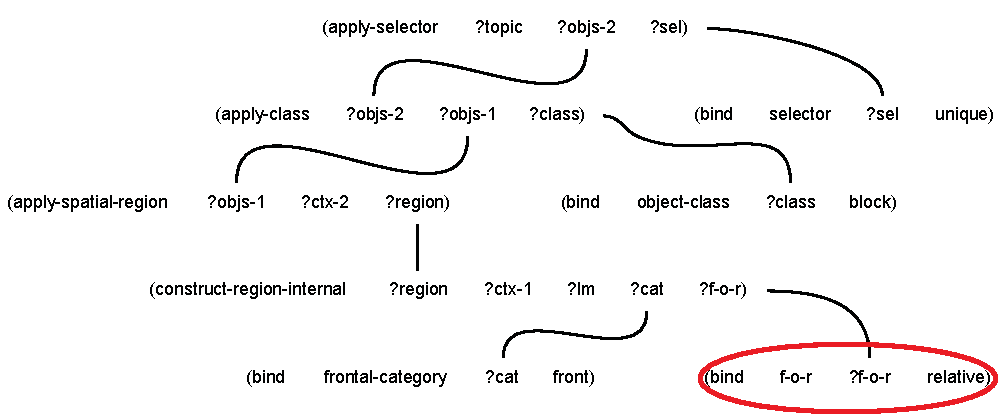
\includegraphics[width=.8\columnwidth]{figs/der-block-vorne-semantic-structure-relative}
\caption[Semantic structure of \textit{der Block vorne} (`the block in front') -- relative]{%
Semantic structure of \textit{der Block vorne} with relative reading. The 
difference from an intrinsic reading is only in the bind statement referring 
to the frame of reference used in computation.}
\label{f:der-block-vorne-semantic-structure-relative}
\end{center}
\end{figure}

\subsubsection{Representing ambiguity in the transient structure}\index{transient structure}
The next question is how the semantic ambiguity\index{semantic ambiguity} and, in particular, the
uncertainty about which interpretation is possible, can be represented 
in syntactic processing. For this, uncertainty has to be represented in the 
transient structure. Uncertainty is represented using a variable. 
Since the procedural IRL-networks have the same convention for variables, 
namely, that variables begin with a {\footnotesize\tt ?}, parts of the 
semantic structure can be replaced using a variable. 
In order to allow FCG to contribute information to those parts in the semantic 
structure that are uncertain or ambiguous, the same variable is repeated in the 
construction. Below as an example is the functional construction for frontal adverbs:

\ea
\label{e:def-fun-frontal-adverb}
%\begin{footnotesize}
\begin{lstlisting}
(def-fun-cxn frontal-adverb 
 (def-fun-skeleton frontal-adverb
  :meaning (== (construct-region-internal 
              ?target ?source ?landmark ?category ?f-o-r)
                      (bind f-o-r ?f-o-r ?f-o-r-value))
  :args ((ref ?target)(src ?source)
           (cat ?category)(landmark ?landmark))
  :sem-function modifier
  :sem-class (region internal-region relative-region)
  :syn-function adverbial
  :syn-class adverb)
 (add-sem-cat frontal-adverb (f-o-r-value ?f-o-r-value)))
\end{lstlisting}
%\end{footnotesize}
\z

Parts of the semantic structure in Figures~\ref{f:der-block-vorne-semantic-structure-intrinsic} and 
\ref{f:der-block-vorne-semantic-structure-relative} are represented by 
adding them to the meaning of this construction.
In particular, the operation and the frame of reference are part of the 
specification of the functional construction. 
Moreover, the actual frame of reference is left unspecified but is 
represented using the variable {\footnotesize\tt ?f-o-r-value}
instead, and it is this variable that is repeated as a semantic category 
attribute. Consequently, this specification
expresses two things: firstly, when a frontal projective category is 
expressed using an adverb, its 
meaning is to construct a region, and, secondly, the frame of reference used 
to construct this region is unspecified.
To summarize, the use of the same variable allows for the representation 
of the uncertainty in a unified way in the semantic structure 
as well as in the construction and, consequently, in the transient structure.

\subsubsection{Constructions for processing semantic ambiguity}\index{semantic ambiguity}
With the knowledge of how to represent semantic structure as well as the 
ambiguity in the semantic interpretation, 
I can now turn to the processing of potentially ambiguous utterances.
I focus first on the ambiguous case only, that is, the case where no 
perspective marker is present in the 
phrase. Consequently, I am trying to solve the problem of 
letting FCG compute all possible interpretations of a
phrase like the one in \REF{e:der-block-vorne-repeated}. 
The key property of the FCG search for an interpretation 
of such an utterance is that each branch in the search tree corresponds 
precisely to one possible interpretation. As a result,
in order to represent the different interpretations of the phrase, the search tree 
must be split, yet it should only split into different branches at the very end of parsing. 
From a processing point of view such a late split is desirable, since branching the 
search at the end reduces computational complexity. From the point of view of modeling, 
it is necessary, because it is only when considering the larger semantic structure
that the phrase can be determined to be ambiguous. In other words, to be sure about 
whether or not the phrase is really ambiguous, processing must be complete 
with no perspective marker observed.

To achieve these objectives, sem-sem constructions are used which
are constructions that only work on the semantic side of the transient structure.
Two of these constructions are needed, one for representing intrinsic readings and 
one for representing relative readings. 
These constructions apply at the very end of parsing, and their job is to set the frame of reference variable.
Here is one of the two sem-sem constructions:
\ea
\label{e:def-sem-sem-intrinsic}
%\begin{footnotesize}
\begin{lstlisting}
(def-sem-sem-cxn 
 :meaning  (== (bind f-o-r ?target intrinsic))
 :sem-cat (==1 (f-o-r-value intrinsic)))
\end{lstlisting}
%\end{footnotesize}
\z
The construction directly applies to the part of the transient 
structure that represents the meaning of the frontal
adverb. Since the {\footnotesize\tt f-o-r-value} was set to the variable {\footnotesize\tt ?f-o-r-value}, this part of the 
transient structure unifies with {\footnotesize\tt intrinsic} and sets the attribute 
as well as the part of the bind statement
in the meaning to the value {\footnotesize\tt intrinsic}. A similar construction is 
used for applying a relative frame of reference. \figref{f:parsing-search-tree-der-block-vorne} shows the split at the end 
of parsing the phrase \textit{der block vorne}.
These constructions are necessarily very general and apply equally to 
all other required cases, in particular to projective prepositions (i.e. frontal and 
lateral prepositions), but also to lateral adverbs.

\begin{figure}
\begin{center}
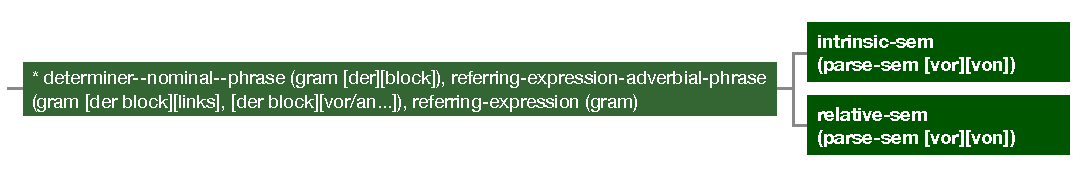
\includegraphics[width=\columnwidth]{figs/parsing-search-tree-der-block-vorne} 
\caption[Parsing semantically ambiguous phrases]{%
Final part of the parsing search tree for the utterance \textit{der block vorne}. 
sem-sem constructions apply at the very end and split the search tree, so 
that the two possible interpretations of the phrase are found.}
\label{f:parsing-search-tree-der-block-vorne}
\end{center}
\end{figure}

The usage of logic variables allows for the representation of the 
uncertainty in interpretation directly in the transient 
structure. In interaction with semantic rules these variables are used 
in processing to provide the different semantic
interpretations of ambiguous German locative phrases.

\subsubsection{Handling perspective markers}
Perspective markers pose a problem in terms of processing, since 
information about perspective marking 
is available on the phrasal level only. For instance, in  
\REF{e:der-block-vor-der-kiste-von-dir-aus}, the
part \textit{vor der Kiste von dir aus} (`in front of the box from your perspective'), 
the perspective marker is the additional phrase \textit{von dir aus}, which together 
with the prepositional phrase in the beginning
makes up the complete phrase. As a consequence, the problem to be solved 
is to distribute the information about the used frame of reference so that a 
construction combining the two phrases
can make the necessary semantic inference, namely, set the frame of reference. 
The information needs to spread all the way to the part of the semantic structure 
processing the region, that is, the functional unit representing the preposition or adverb. 
The answer to this problem is the use of percolation \citep{steels2011phrasal,steels2011design}\index{Steels, L.} 
for distributing the information, so that the information becomes available at
the places necessary. 

Before looking at percolation in more detail, consider \REF{e:der-block-vorne-von-dir-aus}, a simple example where a 
stand-alone adverb is perspective marked (i.e. an adverb that has no landmark 
phrase attached to it).
\ea
\label{e:der-block-vorne-von-dir-aus}
\gll der Block vorne von dir aus\\
the.{\NOM} block.{\NOM} front.{\ADV}  from.{\PREP} your.{\DAT} from.{\PREP}\\ 
\glt `The block in the front of the box from your perspective'\\
%\glend
\z\todo{Please re-consider glossing here and in similar Examples}
Basically, a construction setting the frame of reference to relative is required.
The prerequisite for which is that there is a region that has the potential to be
interpreted as a relative region. Additionally, there needs to be a perspective 
marker that has the right syntactic relationship to the region.
The construction in \figref{f:setting-f-o-r-before} and \REF{e:def-phrasal-relative-region-perspective-marked} does exactly that.

\begin{figure}
\begin{center}
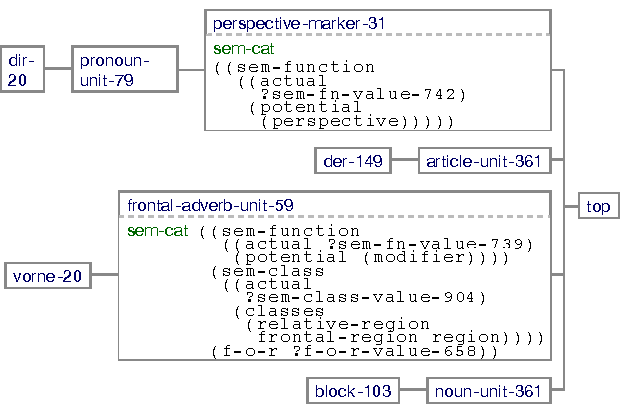
\includegraphics[width=0.8\columnwidth]{figs/perspective-marking-parsing-vorn-von-dir-aus-before} 
\caption[Transient structure before application]{%
Transient structure\index{transient structure} before the application of 
the {\footnotesize\tt relative-region--perspective-marked} construction
(when parsing \textit{der Block vorne von dir aus}). The {\footnotesize\tt f-o-r} 
(frame of reference) {\footnotesize\tt sem-cat} attribute of the 
{\footnotesize\tt frontal-adverb-unit-59} is set to a variable. Consequently, 
at this point in processing it is undetermined which
frame of reference is used. For simplification, 
only the {\footnotesize\tt sem-cat} features of relevant units 
are shown.}
\label{f:setting-f-o-r-before}
\end{center}
\end{figure}

\ea
\label{e:def-phrasal-relative-region-perspective-marked}
%\begin{footnotesize}
\begin{lstlisting}
(def-phrasal-cxn relative-region--perspective-marked
 (def-phrasal-skeleton 
  relative-region--perspective-marked
 :phrase (?relative-region--perspective-marked
              :sem-function (modifier)
              :sem-class (region)
              :syn-function (adverbial)
              :cxn-form (== (meets ?relative-region-unit 
                             ?perspective-marker-unit)))
 :constituents
 ((?relative-region-unit
   :sem-function-potential (modifier)
   :sem-class-potential (relative-region))
  (?perspective-marker-unit
   :sem-function-potential (modifier)
   :sem-class-potential (perspective-marker))))
  (def-set-cat ?relative-region-unit sem-cat 
               f-o-r-value relative))
\end{lstlisting}
%\end{footnotesize}
\z

This construction captures all posed constraints. 
For this construction to apply there need to be two constituents. 
One constituent needs to have the {\footnotesize\tt sem-class} potential 
{\footnotesize\tt relative-region}, that is to say, it needs to be
able to be conceived as a relative region. The second constituent needs 
to be a perspective marker. If these conditions are met, 
the construction sets the frame of reference 
value of the region unit to {\footnotesize\tt relative}. Now, in the case of the 
phrase \textit{vorne von dir aus} (`in front from your 
perspective'), the region unit in parsing corresponds to the adverb unit, namely, 
to the unit setup by the adverb functional construction 
(see \REF{e:def-fun-frontal-adverb}). Figures~\ref{f:setting-f-o-r-before} and
\ref{f:setting-f-o-r-after} show the state of the transient structure before and after application of the construction.

The construction that handles the perspective marking of relative regions is very general.
Its does not constrain the syntactic class of its constituents since it is used to
handle not only cases of stand-alone adverbs but also landmark augmented adverbs 
and prepositional phrases. The problem that remains is how uncertainty about 
the frame of reference is spread, so that this construction 
can distribute its decision on the relative frame of reference to the place where
this information is needed to compute the region, namely, the corresponding functional unit. 
The solution is to apply percolation through all intermediate processing steps. 
For instance, when parsing a frontal prepositional phrase,
such as in \textit{vor der Kiste von dir aus} (`in front of the box from your perspective'), the 
functional unit for \textit{vor} first becomes a constituent of the frontal prepositional phrase 
\textit{vor der Kiste}. Subsequently, the unit for the prepositional phrase becomes a constituent of 
the perspective-marked relative region phrase. Consequently, percolation is added
to the {\footnotesize\tt angular-pp-phrase} construction using an 
agreement macro (see \citealp{steels2011phrasal,steels2011design}\index{Steels, L.} for details).

\begin{figure}
\begin{center}
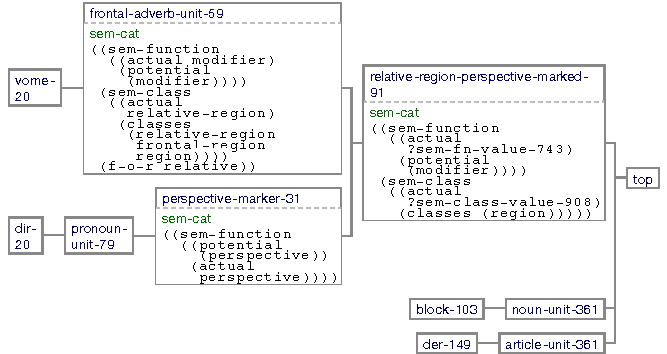
\includegraphics[width=0.8\columnwidth]{figs/perspective-marking-parsing-vorn-von-dir-aus-after} 
\caption[Transient structure after application]{Transient structure after the application 
of the {\footnotesize\tt relative-region--perspective-marked} construction
(when parsing \textit{der Block vorne von dir aus}). The {\footnotesize\tt f-o-r} (frame of reference) {\footnotesize\tt sem-cat} attribute of the 
{\footnotesize\tt frontal-adverb-unit-59} is set to {\footnotesize\tt relative} and therefore determined.}
\label{f:setting-f-o-r-after}
\end{center}
\end{figure}

\ea
\label{e:def-angular-pp-phrase-agreement}
%\begin{footnotesize}
\begin{lstlisting}
(def-add-phrasal-agreement angular-pp-phrase
 (?relative-region-unit
  :sem-cat (f-o-r-value ?f-o-r-value)
 (?angular-pp-unit
  :sem-cat (f-o-r-value ?f-o-r-value)))
\end{lstlisting}
%\end{footnotesize}
\z
Similarly, this scheme has to be applied to landmark augmented adverbs in order for them to participate
in these solutions.

Using a collection of techniques such as logic variables, percolation and a sem-sem 
of construction (that only operate on the semantic side), we are able
to model the interaction of projective categories with perspective marking and their 
effects on semantic ambiguity pervasive in German locative phrases. 

\subsection{Semantic processing}
\label{s:semantic-ambiguity-semantic}
The second part of handling semantic ambiguity\index{semantic ambiguity} is in interpretation. 
Let us consider the following phrase.
\ea
\label{e:der-block-vor-der-kiste-repeated}
\gll der Block vor der Kiste \\
the.{\NOM} block.{\NOM} front.{\PREP} the.{\DAT} box.{\DAT} \\
\glt `The block in front of the box'\\
%\glend
\z
This phrase has an intrinsic and a relative reading. Consequently, FCG finds
those two readings and passes them as potential solutions to IRL. 
The task engine splits in search which allows to trace each of the two interpretations
separately (see \figref{f:processing-interpretations}).

Suppose that a speaker uttered this phrase in the spatial scene 
shown in \figref{f:scene} (which is repeated here in \figref{f:scene-repeated}) and he wants to refer to object {\footnotesize\tt obj-266} in his context (which
is {\footnotesize\tt obj-253} in the hearer's context). 
In this scene there are at least three possible conceptualizations of the
scene which are compatible with the information conveyed in the utterance. 
One is the intrinsic interpretation. The other two are variants of the relative
interpretation. Relative conceptualizations of spatial scenes depend on perspective.
The scene has two robots which both could in principle be used as perspective.
IRL recovers all three conceptualizations of the scene. The hearer can then
choose which of the interpretations is the best one (see \figref{f:interpretations} for a
depiction of the three possible interpretations and \figref{f:processing-interpretations} for
an overview of processing). The final decision is based 
on the discrimination score of the three possible interpretations.

In this particular configuration all three interpretations lead 
to different results. This is not always the case. There are three 
ways of dealing with semantic ambiguity.
\begin{itemize}
\item The speaker detects that the phrase would be ambiguous in re-entrance\index{re-entrance} and 
chooses to avoid the problem by expressing himself differently.
\item  In some scenes even though a phrase might be highly ambiguous with 
many different interpretations, all of these interpretations refer to the same object.
In this case disambiguation becomes unnecessary. An example where this happens
are certain vertical relations for which intrinsic, absolute and 
relative interpretations often overlap
\citep{carlson1999selecting}\index{Carlson, L. A.}.
\item The speaker relies on the interpretation power of the hearer. This happened in
the case study discussed in this section. For this particular scene the interaction was
a success and the hearer correctly identified the topic.
\end{itemize}
Importantly, in all three cases agents rely on the power of IRL and FCG 
to deal with semantic ambiguity\index{semantic ambiguity}.


\begin{figure}[p]
\begin{center}
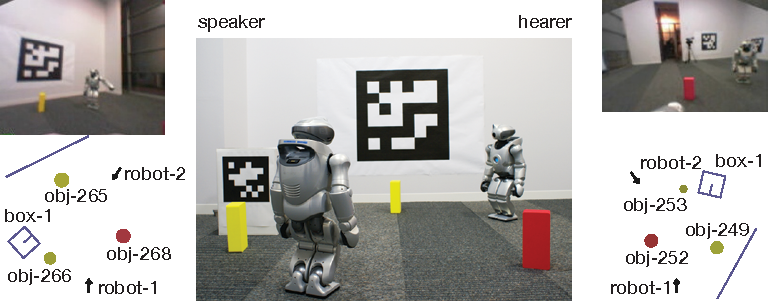
\includegraphics[width=0.8\columnwidth]{figs/space-scene-2-small}
\end{center}
\caption[Example scene]{Example scene (same as in \figref{f:scene}).}
\label{f:scene-repeated}
\end{figure}

\begin{figure}[p]
\begin{center}
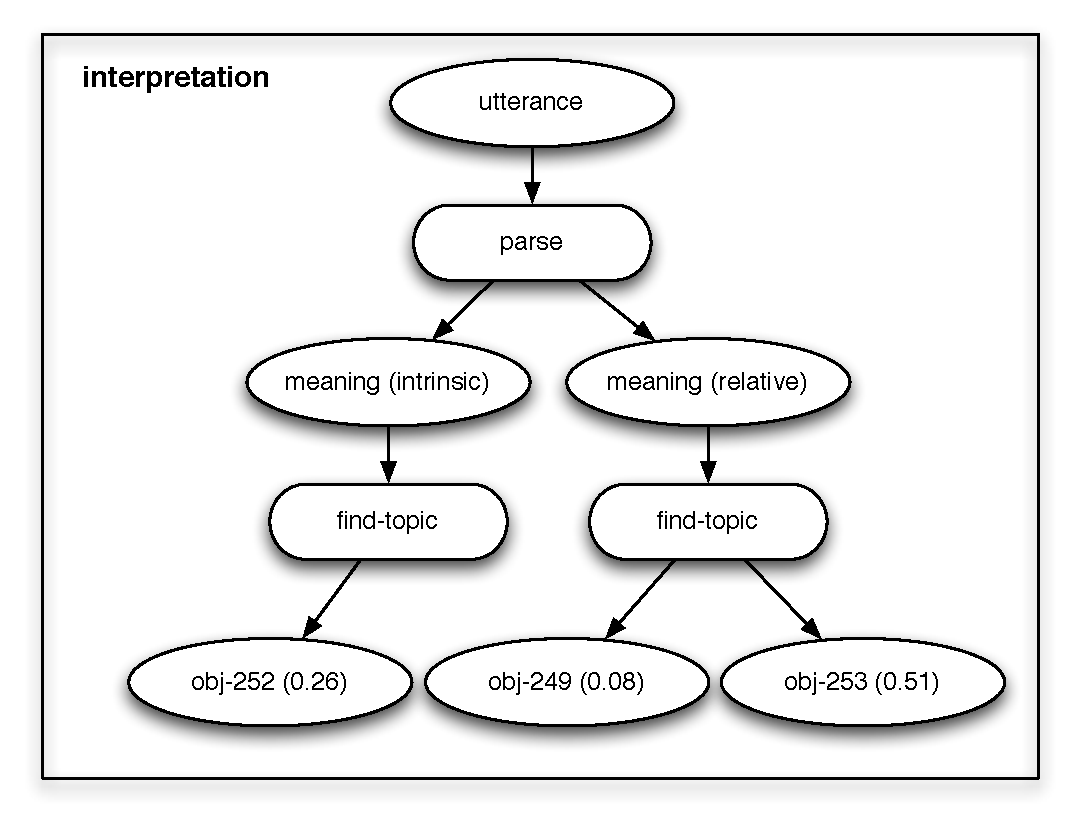
\includegraphics[width=0.5\columnwidth]{figs/semantic-ambiguity-interpretation}
\end{center}
\caption[Interpretation example schematic]{%
Interpretation of \REF{e:der-block-vor-der-kiste-repeated}. In parsing,
FCG finds two possible interpretations (relative and intrinsic). IRL is then called 
on each of these interpretations separately and recovers 
two possible conceptualizations for the relative reading. All three
possible interpretations and their corresponding topics are scored. 
The hearer then decides that {\footnotesize\tt obj-253} is the best interpretation.}
\label{f:processing-interpretations}
\end{figure}
\clearpage
\begin{figure}[t]
\begin{center}
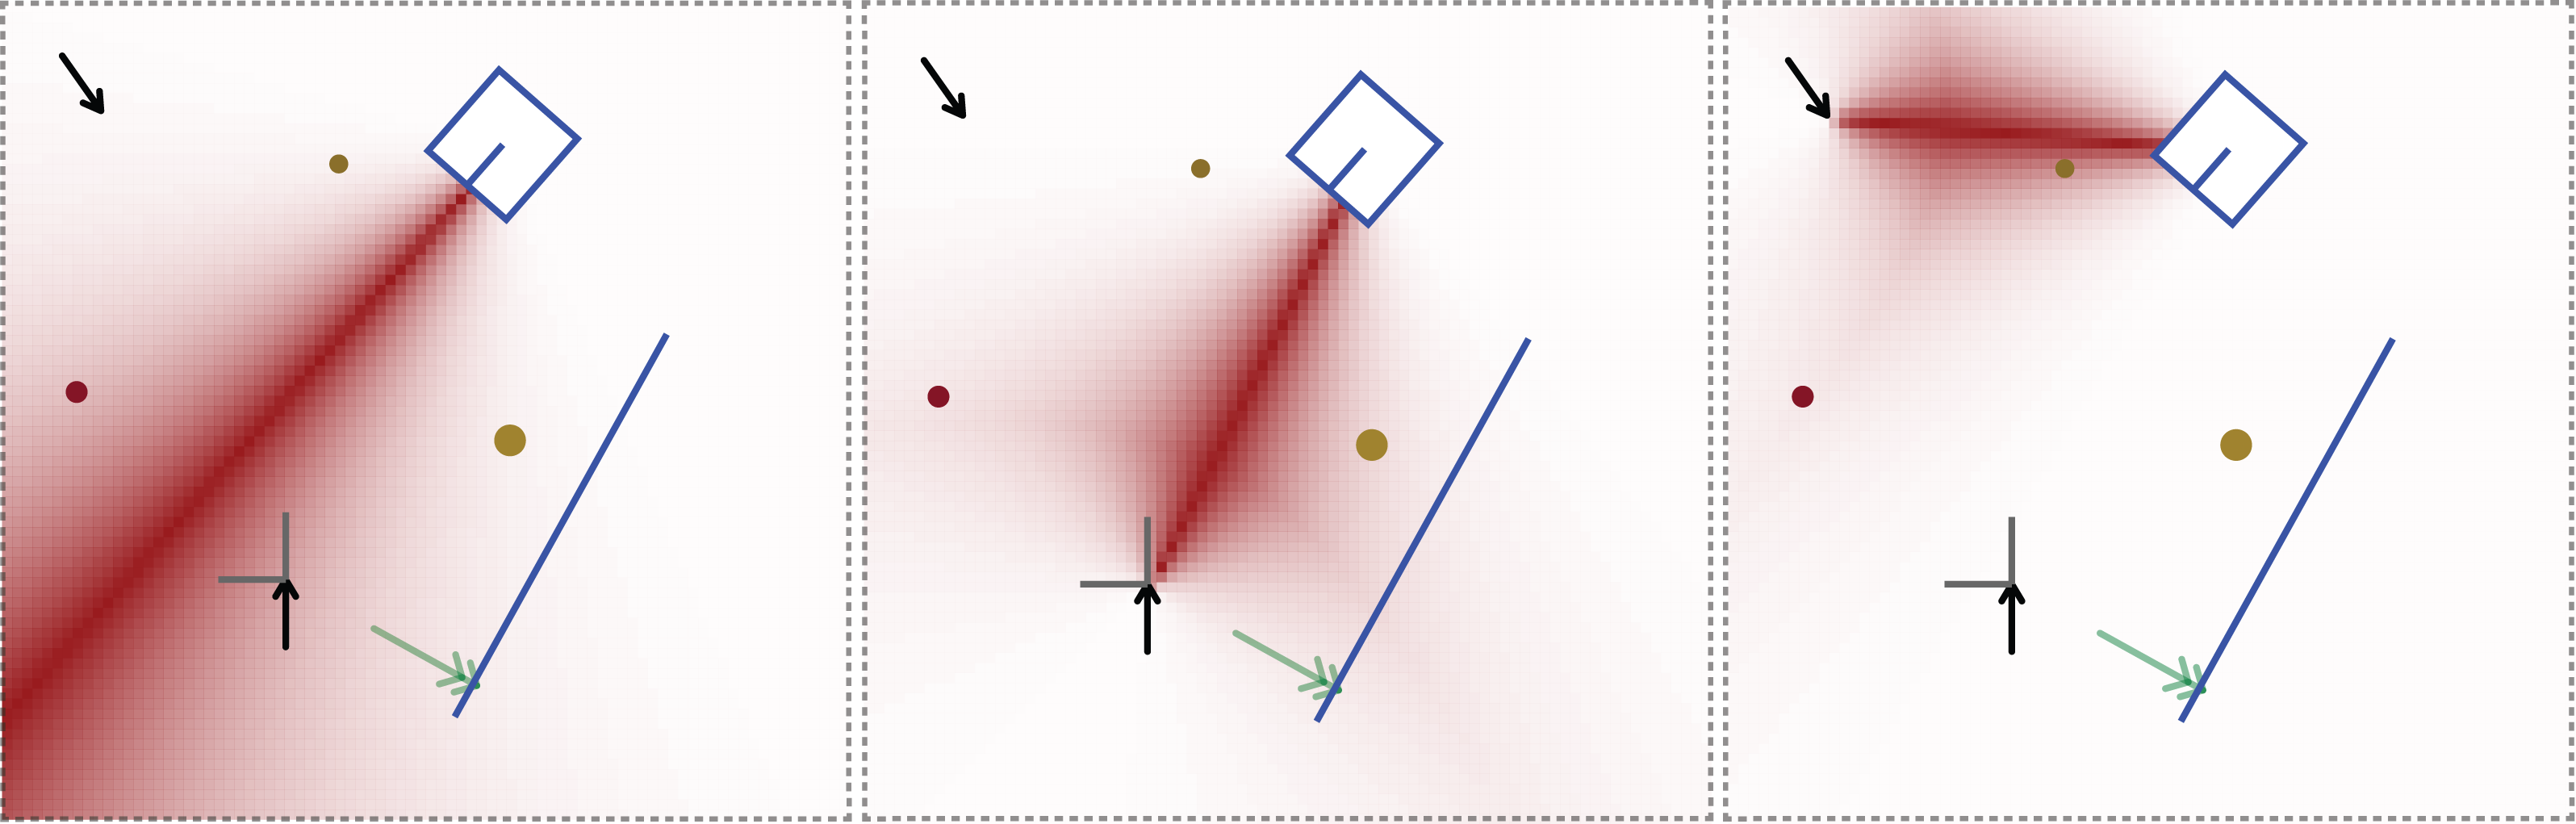
\includegraphics[width=0.95\columnwidth]{figs/semantic-ambiguity-interpretations.png}
\end{center}
\caption[Interpretation example graphic]{Possible interpretations of \REF{e:der-block-vor-der-kiste-repeated}.
From left to right (1) intrinsic interpretation, (2) relative from the perspective of the hearer,
and (3) relative from the perspective of the speaker. All of these interpretations have
different topics. The intrinsic representation evaluates to object {\footnotesize\tt obj-252},
the relative interpretation from the hearer evaluates to {\footnotesize\tt obj-249}, and
the relative interpretation from the speaker to {\footnotesize\tt obj-253}.}
\label{f:interpretations}
\end{figure}


\section{Discussion and results}
\label{s:syntax+semantics-integration}
We can now test the complete system and see how it performs
on different spatial scenes. Figure \ref{f:interpretations} compares the average success 
of agents in varying environmental conditions. Agents play 20000 language
games. After each of the games the success is measured. If the interaction 
was a success then a 1.0 is recorded, 0.0 otherwise. The German locative system 
is quite successful in the three conditions: ``similar perspective'', 
``no box landmark'' and ``many objects''. In the first condition, the 
perspective of agents is similar and the number of objects is reasonable.
The ``no box landmark'' condition is one where in every scene there are only the two
robots available as landmarks. The third condition features varied perspective of the two
robots on the scene. Most importantly, there are many objects in every scene in this condition .
The system performs worst in the ``many objects'' condition, but overall copes 
well even with the complex ``many objects'' scenes.

These results suggest that the complete system works reliably and allows agents
to talk about objects in their environment using German locative phrases and
validates in some respect the reconstructed syntactic and semantic processing 
as well as the perception system. The results show the power of the whole systems approach.
Success is high even in difficult scenes where humans would have trouble finding appropriate
phrases.

\begin{figure}
\begin{center}
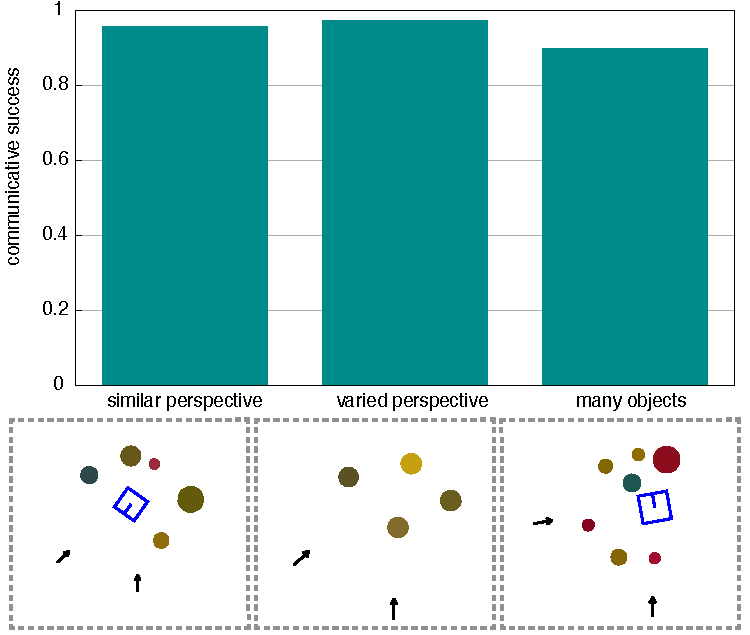
\includegraphics[width=.8\columnwidth]{figs/results-german-grammar}
\end{center}
\caption[Average success of agents operating the German locative system]{%
Average success of agents operating the German locative grammar
and semantics in different spatial scenes.}
\label{f:interpretations}
\end{figure}


%\bibliographystyle{diss}
%\bibliography{papers,space} 
%\end{document}